\documentclass{ximera}

\graphicspath{{./graphics/}{./content/04_4_local_extrema/graphics/}}

\title{Local Extrema}
\begin{document}
\begin{abstract}
\end{abstract}
\maketitle

Now that we've defined the Hessian matrix and studied quadratic forms, we're in position to find local extrema of multivariable function. This process will closely resemble the process that we following in single variable calculus, so we'll begin by reviewing that case.

Recall that we say $f(x)$ has a local maximum at $x=a$ if $f(x)\leq f(a)$ for all $x$ near $a$. Similarly, $f(x)$ has a local minimum at $x=a$ if $f(a)\leq f(x)$ for all $x$ near $a$. We can state these definitions more precisely, as below.

\begin{definition}
We say that $f(x)$ has a \emph{local maximum} at $x=a$ if there exists $r>0$ such that $|x-a|<r$ implies $f(x)\leq f(a)$.

We say that $f(x)$ has a \emph{local minimum} at $x=a$ if there exists $r>0$ such that $|x-a|<r$ implies $f(x)\geq f(a)$.
\end{definition}

In single variable calculus, we found local extrema by finding critical points, and then classifying them using the first or second derivative test.

\begin{definition}
The point $x=a$ is a \emph{critical point} of $f(x)$ if $f'(a)=0$, or if $f'(a)$ does not exist.
\end{definition}

\begin{proposition}
If $f(x)$ has a local minimum or maximum at $x=a$, then $a$ is a critical point of $f(x)$.

If $a$ is a critical point of $f(x)$ and $f''(a)<0$, then $f(x)$ has a local maximum at $x=a$.

If $a$ is a critical point of $f(x)$ and $f''(a)>0$, then $f(x)$ has a local minimum at $x=a$.

If $a$ is a critical point of $f(x)$ and $f''(a)=0$ or $f''(a)$ does not exist, then $f(x)$ could have a local maximum at $a$, a local minimum at $a$, or neither.
\end{proposition}

\begin{example}
As an example, we'll find the local extrema of the function $f(x) = x^3+3x^2-9x+1$. Differentiating, we have
\[
f'(x) = \answer{3x^2+6x-9}.
\]
Solving $f'(x)=0$ for $x$, we see that there are two critical points, $x=-3$ and $x=1$.

We'll classify these critical points using the second derivative test. We find the second derivative of $f(x)$.
\[
f''(x) = \answer{6x+6}
\]
Plugging in $x=-3$, we have
\[
f''(-3) = \answer{-12}.
\]
This tells us that at $x=-3$, $f(x)$ has a
\begin{multipleChoice}
\choice[correct]{local maximum.}
\choice{local minimum.}
\choice{neither.}
\end{multipleChoice}
Plugging in $x=1$, we have
\[
f''(1) = \answer{12}.
\]
This tells us that at $x=1$, $f(x)$ has a
\begin{multipleChoice}
\choice{local maximum.}
\choice[correct]{local minimum.}
\choice{neither.}
\end{multipleChoice}
\end{example}

\section*{Local extrema for multivariable functions}

We begin by defining local minima and local maxima for multivariable functions. These follow the same idea as in the single variable case. For example, $f$ has a local minimum at $\vec{x}=\vec{a}$ if $f(\vec{a})\leq f(\vec{x})$ for $\vec{x}$ ``near'' $a$. Now, we need to decide what ``near'' means. This means that we can find some distance $r>0$ such that for $\vec{x}$ within distance $r$ from $\vec{a}$, we must have $f(\vec{a})\leq f(\vec{x})$. We restate this more formally.

\begin{definition}
We say that $f:\mathbb{R}^n\rightarrow\mathbb{R}$ has a \emph{local minimum} at $\vec{x}=\vec{a}$ if there exists $r>0$ such that for all $\vec{x}$ with $\|\vec{x}-\vec{a}\|<r$, we have $f(\vec{a})\leq f(\vec{x})$.

We say that $f:\mathbb{R}^n\rightarrow\mathbb{R}$ has a \emph{local maximum} at $\vec{x}=\vec{a}$ if there exists $r>0$ such that for all $\vec{x}$ with $\|\vec{x}-\vec{a}\|<r$, we have $f(\vec{a})\geq f(\vec{x})$.
\end{definition}

In some cases, we can determine local extrema using our knowledge about functions, and without using Calculus.

\begin{example}
Consider the function $f(x,y)= (x-1)^2 + (y+2)^2$. Since the terms $(x-1)^2$ and $(y+2)^2$ are always nonnegative, we can see that $f(x,y)$ will always be nonnegative. Since $f(1,-2)=0$, and $0\leq f(x,y)$ for all $(x,y)$, this means that $f(x,y)$ has a local minimum at $(1,-2)$. (This local minimum is also an absolute maximum.)

Consider the function $g(x,y,z) = 1-\sqrt{x^2+y^2+z^2}$. Since $\sqrt{x^2+y^2+z^2}\geq 0$, we'll always have $g(x,y,z) \leq 1$. Then, since $g(0,0,0)=1$, $g$ has a local maximum at $(0,0,0)$.
\end{example}

\section*{Critical points}

Our definition of critical points of multivariable functions is also very similar to the definition from single variable calculus. Here, the gradient vector replaces the derivative.

\begin{definition}
We say that $f:\mathbb{R}^n\rightarrow\mathbb{R}$ has a \emph{critical point} at $\vec{x}=\vec{a}$ if $\nabla f(\vec{a})=\vec{0}$, or $\nabla f(\vec{a})$ does not exist.
\end{definition}

For functions $f:\mathbb{R}^2\rightarrow\mathbb{R}$, we can visualize critical points as points where the tangent plane is either horizontal, or undefined. Each of the graphs below has a critical point at $(0,0)$.

\begin{image}
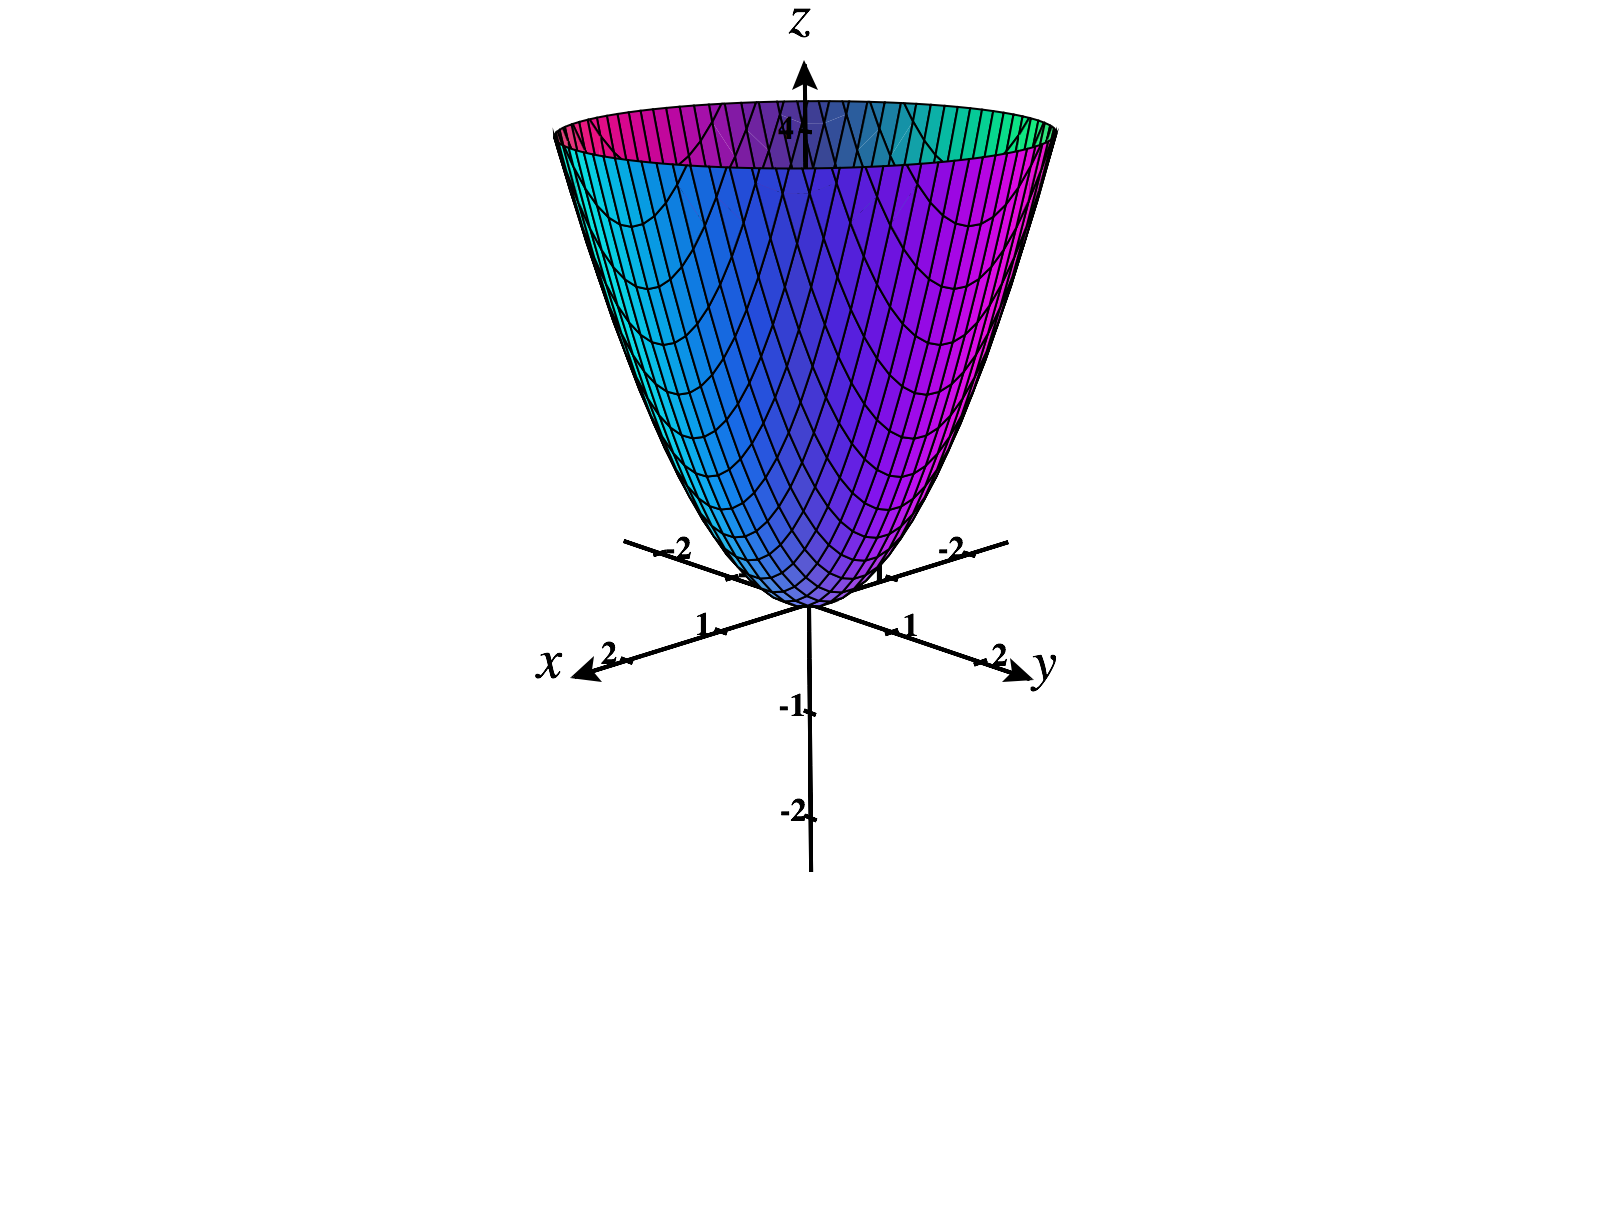
\includegraphics[width = .33\textwidth]{CalcPlot3D-pos_def}
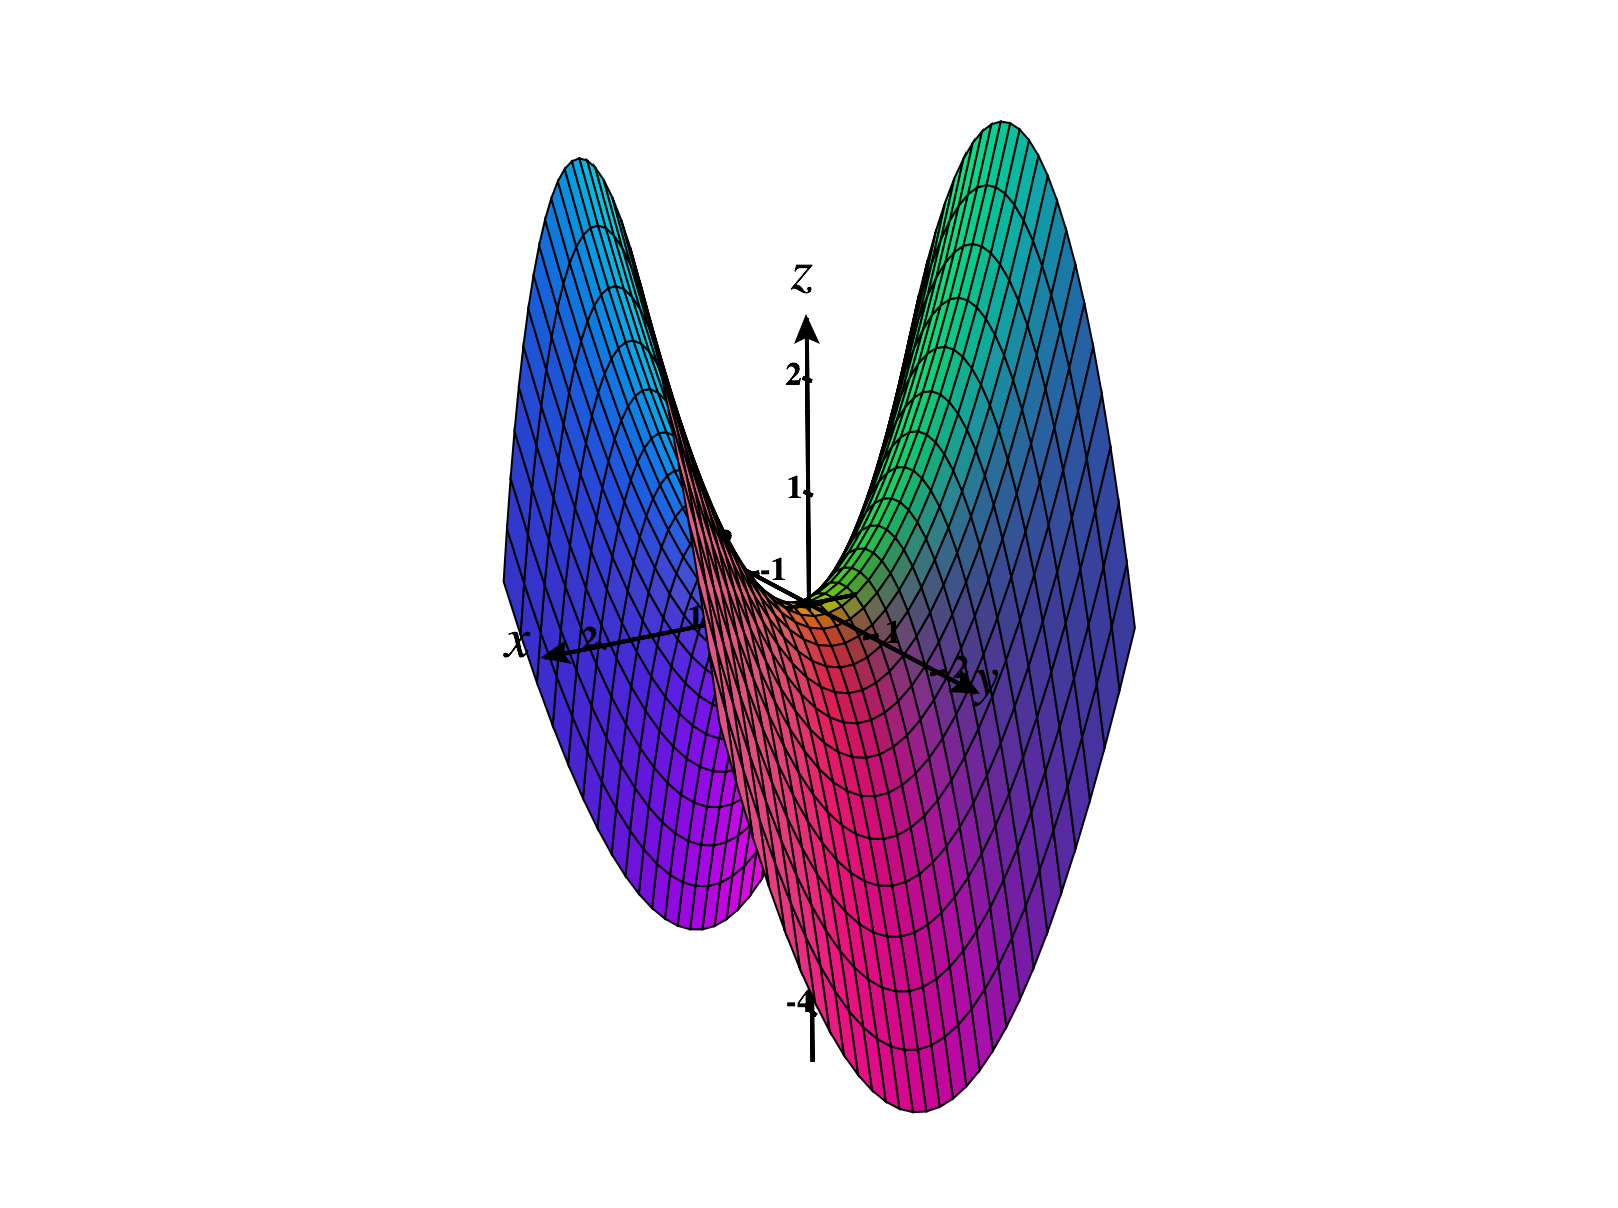
\includegraphics[width = .33\textwidth]{CalcPlot3D-indef}
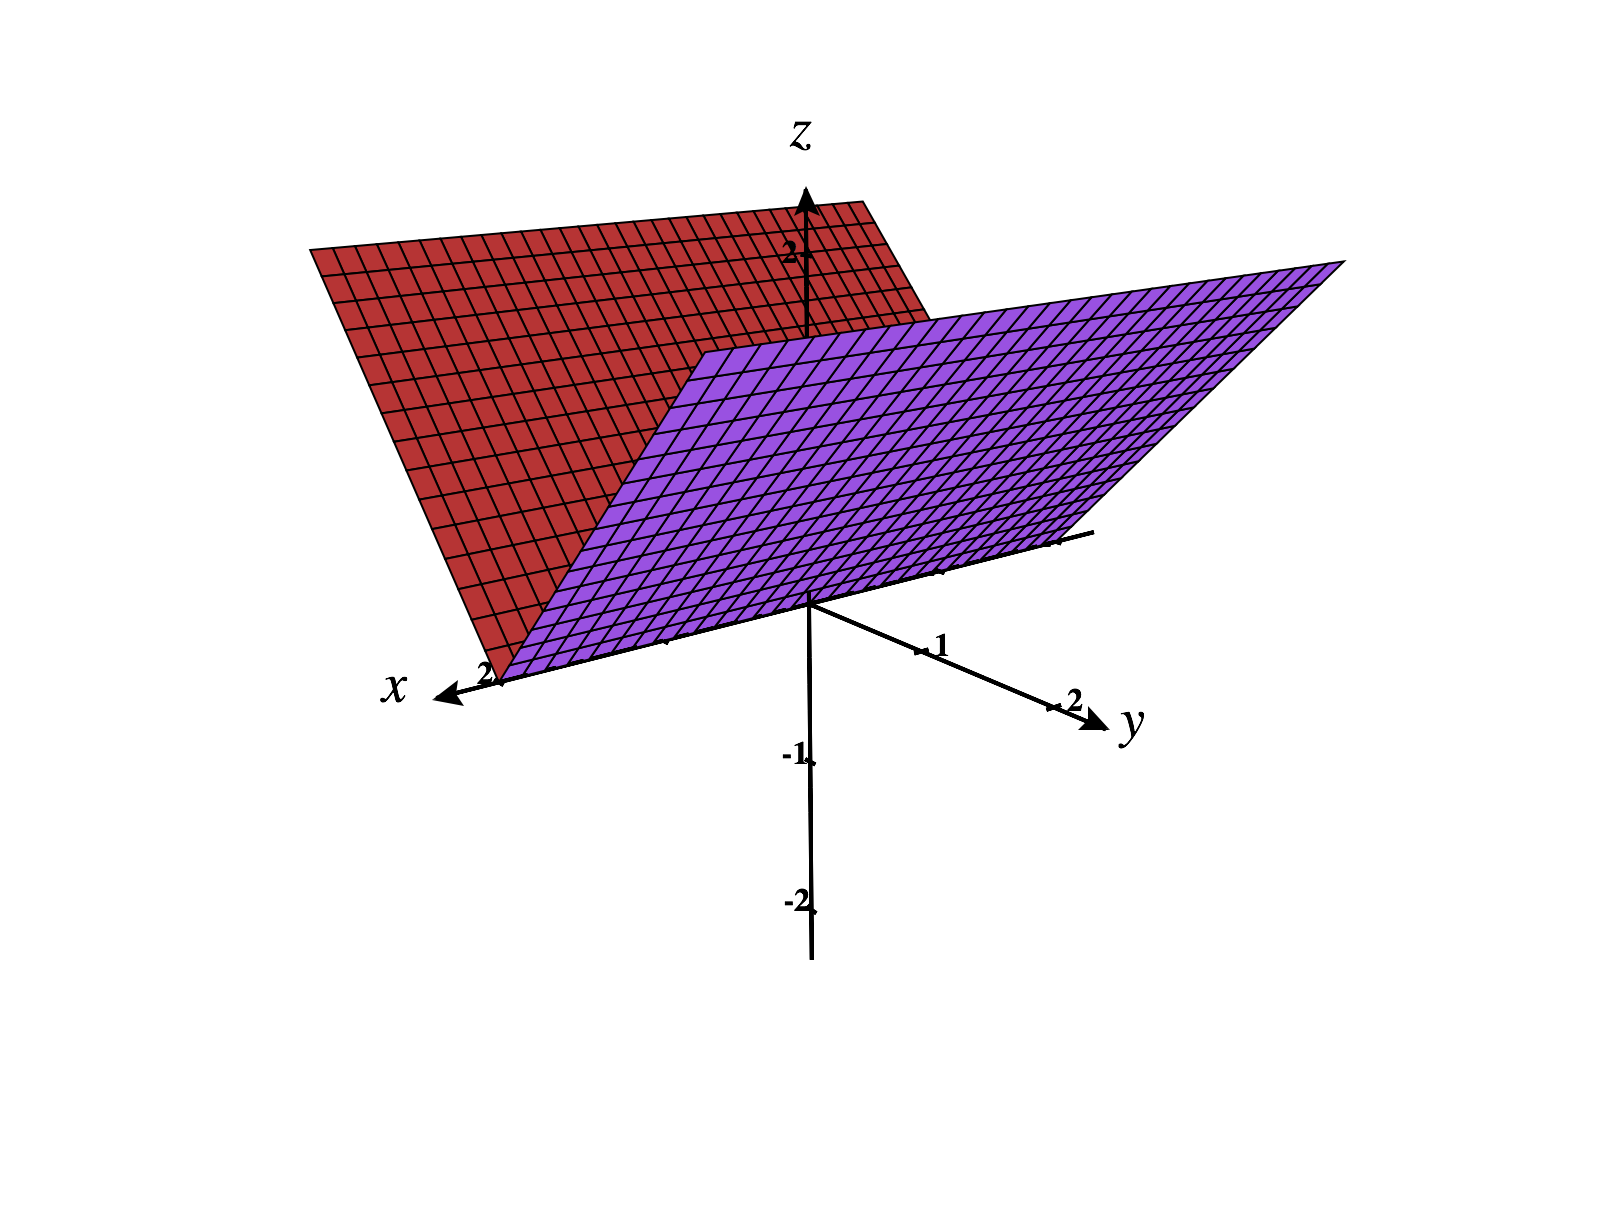
\includegraphics[width = .33\textwidth]{CalcPlot3D-abs}
\end{image}

As in single variable calculus, if a function has local extrema, they will occur at critical points.

\begin{proposition}
If $f:\mathbb{R}^n\rightarrow\mathbb{R}$ has a local maximum or local minimum at $\vec{x}=\vec{a}$, then $\vec{a}$ is a critical point of $f$.
\end{proposition}

\begin{example}
We'll find the critical points of the function $f(x,y) = x^3+x^2y-y^2-4y$. The gradient of $f$ is
\[
\nabla f(x,y) = (3x^2+2xy, x^2-2y-4).
\]
This is defined at all points in $\mathbb{R}^2$, so the critical points will satisfy $\nabla f(x,y)=(0,0)$. In order to find the critical points, we solve the system of equations
\[\begin{cases}
3x^2+2xy=0\\
x^2-2y-4=0
\end{cases}.\]
Factoring the first equation, we have $x(3x+2y)=0$, giving us the cases $x=0$ or $3x+2y=0$.

If $x=0$, the second equation gives us $y=-2$. So $(0,-2)$ is a critical point.

If $3x+2y=0$, plugging $y=\frac{-3}{2} x$ into the second equation gives us $x^2+3x-4=0$, so $x=1$ or $x=-4$. This gives us the critical points $(1,-3/2)$ and $(-4,6)$.

Thus, the critical points of $f$ are $(0,-2)$, $(1,-3/2)$, and $(-4,6)$.
\end{example}

\section*{Classifying critical points}

Analogous to the second derivative test from single variable calculus, we can use the Hessian matrix to classify critical points in some cases.

\begin{proposition}
Suppose $f:\mathbb{R}^n\rightarrow\mathbb{R}$ has continuous second order partial derivatives (so $f$ has $\mathcal{C}^2$) at and near a critical point $\vec{a}\in U$.
\begin{itemize}
\item If $Hf(\vec{a})$ is positive definite, then $f$ has a \emph{local minimum} at $\vec{x}=\vec{a}$.
\item If $Hf(\vec{a})$ is negative definite, then $f$ has a \emph{local maximum} at $\vec{x}=\vec{a}$.
\item If $Hf(\vec{a})$ is indefinite, then $f$ has a saddle point at $\vec{x}=\vec{a}$.
\end{itemize}
\end{proposition}

\begin{example}
Consider again the function $f(x,y) = x^3+x^2y-y^2-4y$. Earlier, we found the critical points of this function, which are $(0,-2)$, $(1,-3/2)$, and $(-4,6)$. In order to classify these critical points, we find the Hessian matrix of $f$.
\[
Hf(x,y) = \begin{pmatrix}
\answer{6x+2y} & \answer{2x}\\
\answer{2x} & \answer{-2}
\end{pmatrix}
\]
Plugging in the point $(0,-2)$, we have
\[
Hf(0,-2) = \begin{pmatrix}
\answer{-4} & \answer{0}\\
\answer{0} & \answer{-2}
\end{pmatrix}.
\]
Using Sylvester's Theorem, we can see that $Hf(0,-2)$ is
\begin{multipleChoice}
\choice{positive definite.}
\choice[correct]{negative definite.}
\choice{indefinite.}
\choice{we cannot determine this using Sylvester's Theorem.}
\end{multipleChoice}
This means that, at $(0,-2)$, $f(x,y)$ has a
\begin{multipleChoice}
\choice[correct]{local maximum.}
\choice{local minimum.}
\choice{saddle point.}
\choice{none of the above.}
\end{multipleChoice}
Next, we'll classify the critical point $(1,-3/2)$. We find the Hessian matrix at this point,
\[
Hf(1,-3/2) = \begin{pmatrix}
\answer{3} & \answer{2}\\
\answer{2} & \answer{-2}
\end{pmatrix}.
\]
Using Sylvester's Theorem, we can see that $Hf(1,-3/2)$ is
\begin{multipleChoice}
\choice{positive definite.}
\choice{negative definite.}
\choice[correct]{indefinite.}
\choice{we cannot determine this using Sylvester's Theorem.}
\end{multipleChoice}
This means that, at $(1,-3/2)$, $f(x,y)$ has a
\begin{multipleChoice}
\choice{local maximum.}
\choice{local minimum.}
\choice[correct]{saddle point.}
\choice{none of the above.}
\end{multipleChoice}
Finally, we'll classify the critical point $(-4,6)$. We find the Hessian matrix at this point,
\[
Hf(-4,6) = \begin{pmatrix}
\answer{-12} & \answer{-8}\\
\answer{-8} & \answer{-2}
\end{pmatrix}.
\]
Using Sylvester's Theorem, we can see that $Hf(-4,6)$ is
\begin{multipleChoice}
\choice{positive definite.}
\choice{negative definite.}
\choice[correct]{indefinite.}
\choice{we cannot determine this using Sylvester's Theorem.}
\end{multipleChoice}
This means that, at $(-4,6)$, $f(x,y)$ has a
\begin{multipleChoice}
\choice{local maximum.}
\choice{local minimum.}
\choice[correct]{saddle point.}
\choice{none of the above.}
\end{multipleChoice}
\end{example}


\end{document}